\documentclass[../main.tex]{subfiles}
\graphicspath{{\subfix{../images/}}}

\begin{document}

\newpage
\chapter{METHODOLOGY}

\section{Overview}

Fdtd Lucuma is a electromagnetic simulator made in C++26.
It can be used from the command line and from a GUI made with Dear ImGui\cite{imgui}.
Internally it is structured using Entity Component System (ECS) and with swappable services using a handwritten dependency injector.
From which the \texttt{frontend} (CLI or GUI) consumes one of the \texttt{backends}.
Currently it has 8 backends, one per each pair of archetype and supported precision:

\begin{table}[H]
	\centering
	\begin{tabular}{l|c|c|c}
		Precision: & float16 & float32 & float64 \\
		\hline
		CPU sequential & \checkmark & \checkmark & \checkmark \\
		CPU parallel   & \checkmark & \checkmark & \checkmark \\
		Vulkan         & \checkmark & \checkmark & \times\footnotemark \\
	\end{tabular}
	\caption{Fdtd Lucuma's backend support matrix}
	\label{tab:nine_backends}
\end{table}
\footnotetext{As of 2026, the Spirv \texttt{exp()} instruction only supports 16-bits and 32-bits\cite{spirv_spec}.}

The sequential backends uses plain C++, while the parallel ones uses Taskflow\cite{Huang_2022}.
For the Vulkan backends, Fdtd Lucuma implements the FDTD method using Vulkan\cite{vulkanspec} Compute Pipelines made from, as shown in Figure \ref{fig:vulkan_compute_pipeline}, shaders written in Shader Slang\cite{10.1145/3197517.3201380}.

% How do I cite this?
Apart from that there is a FDTD implementation in Julia CUDA\cite{besard2018juliagpu} that will only be used as part of Chapter \ref{sec:results} results comparison.

\section{Structure}

\begin{figure}[H]
	\centering
	\begin{tikzpicture}[
			transform shape,
			node distance=1cm,
			stacked/.style={
				double copy shadow={
					shadow xshift=1mm,
					shadow yshift=-1mm,
				}
			},
			vulkan/.style={
				fill=red!30
			}
		]

		\graph[layered layout, components go right top aligned, nodes={draw, fill=green!30}, edges=rounded corners, sibling distance=2cm, layer distance=2cm]{
			Frontends[stacked, label=left:\blackcircle{graph:frontends}] ->
			backends[as={Backends $*$ \{f16,f32,f64\}}, stacked, label=left:\blackcircle{graph:backends}, text width=2.5cm, text centered] ->
			"Basic services"[stacked, label=left:\blackcircle{graph:services}];

			{[same layer] Frontends, CLI, GUI};
			{[same layer] backends, "CPU Sequential", "CPU Parallel", Vulkan[vulkan]};
			{[same layer] "Basic services", "EnTT", "Settings"};

			GUI -> {"CPU Sequential", "CPU Parallel", "Vulkan"};
			CLI -> {"CPU Sequential", "CPU Parallel", "Vulkan"};

			"CPU Sequential" -> {"EnTT", "Settings"};
			"CPU Parallel" -> {"EnTT", "Settings"};
			"Vulkan" -> {"EnTT", "Settings"};

			"EnTT" -> etc[as=Other services$\ldots$, stacked];
			"Settings" -> etc;

			{[same layer] etc, vulkan2[as=Vulkan services$\ldots$, stacked, vulkan]};
			{Vulkan, GUI} -> vulkan2;
		};

	\end{tikzpicture}
	\caption{Fdtd Lucuma's services graph}
	\label{fig:fdtd_lucuma_service_graph}
\end{figure}

As shown in Figure \ref{fig:fdtd_lucuma_service_graph} Fdtd Lucuma is structured in services.
Each one is lazily instantiated the first time one of it's dependents needs to inject it as a dependency.

At the start of the program execution, Fdtd Lucuma instantiates one of it's \blackcircleref{graph:frontends} frontends dependending on the cli arguments used.
The CLI frontend instantiates a single \blackcircleref{graph:backends} backend, while the GUI frontend instantiates the ones that it needs.
Then each backend instantiates the \blackcircleref{graph:services} services that it needs.

\section{Entity Component System}
%As mentioned before, Fdtd Lucuma uses EnTT an Entity Component System library.
EnTT\cite{entt} is the open source C++ header-only library Fdtd Lucuma uses to implement the Entity Component System paradigm.
It provides the \texttt{registry}, an object that has methods to create, update and delete entities and components.
Each entity is used to identify a tuple of components stored inside the registry.
Each component is a struct instance that holds data and its related to an entity.

\begin{table}[H]
	\centering
	\begin{tabular}{l|l|l}
		Entity & Position & GaussianSource \\
		\hline
		0 & x: 1, y:1, z:1 & sigma: 1 \\
		1 & x: 2, y:2, z:2 & sigma: 1 \\
		2 & x: 10, y:10, z:10 & sigma: 2 \\
	\end{tabular}
	\caption{Three Gaussian sources in ECS}
	\label{tab:ecs_example}
\end{table}
\footnotetext{As of 2026, the Spirv \texttt{exp()} instruction only supports 16-bits and 32-bits\cite{spirv_spec}.}

This approach allows for each service (\emph{system}) to iterate and filter over one or more components.
Moreover, each simulation has its own private EnTT registry to avoid data sharing between multiple simulations that run in parallel.

EnTT also provides the \texttt{dispatcher}, which is used by Fdtd Lucuma's services to communicate with each other using signals while also sharing data with EnTT's registry.
The registry is used to store the simulation objects as entities with components as show in Table \ref{tab:ecs_example}, this allows the backends to iterate them in a cache-friendly way because the components are stored in continuous arrays in memory and only the components needed for the logic are fetched instead of wasting L1 cache lines on useless data.


% EnTT
% Cache friendly
% Entities and components
% Data oriented design
% idk

\section{Flow} \label{sec:flow}

\newpage

\begin{figure}[H]
	\centering
	\begin{tikzpicture}[
			transform shape,
			node distance=1cm
		]

		\node[startstop] (start) {Start};

		\node[io, below=of start] (select) {Configure simulation parameters};

		\node[process, below=of select] (services) {\blackcircle{step:services} Start basic services and selected backend. (As shown in Figure \ref{fig:fdtd_lucuma_service_graph})};
		\node[process, below=of services] (entity) {\blackcircle{step:entity} Create a new ECS entity};
		\node[process, below=of entity] (simulation) {\blackcircle{step:state} Attach the simulation state\footnotemark and a private registry with the sources to \blackcircleref{step:entity}};
		\node[decision, below=of simulation, yshift=0.25cm] (while) {time++ < max\_time};


		\node[process, below=of while] (updateH) {\blackcircle{step:magnetic} Update magnetic $H_{\{x,y,z\}}$ fields};
		\node[process, below=of updateH] (updateE) {\blackcircle{step:electric} Update electric $E_{\{x,y,z\}}$ fields};
		\node[process, below=of updateE] (sources) {\blackcircle{step:sources} Apply sources};
		\node[process, below=of sources] (abc) {\blackcircle{step:abc} Apply boundary conditions};

		\node[process, right=2cm of while] (cleanup) {Cleanup \blackcircleref{step:state}, \blackcircleref{step:entity} and \blackcircleref{step:services}};
		\node[startstop, below=of cleanup] (end) {End};

		\draw[arrow] (start) -- (select);
		\draw[arrow] (select) -- (services);
		\draw[arrow] (services) -- (entity);
		\draw[arrow] (entity) -- (simulation);
		\draw[arrow] (simulation) -- (while);
		\draw[arrow] (while) -- node[anchor=south] {No} (cleanup);
		\draw[arrow] (cleanup) -- (end);
		\draw[arrow] (while) -- node[anchor=east] {Yes} (updateH);
		\draw[arrow] (updateH) -- (updateE);
		\draw[arrow] (updateE) -- (sources);
		\draw[arrow] (sources) -- (abc);
		\draw[arrow] (abc.west) -| ++(-2,0) |- (while.west);

	\end{tikzpicture}
	\caption{Simulation flowchart}
	\label{fig:fdtd_lucuma_flow}
\end{figure}

\footnotetext{Parameters and buffers}

\section{CLI frontend}
A simple command line interface that runs a single simulation from the commmand line arguments.
While also being able to run multiple simulations from one or more json files when passed as positional arguments.

\begin{figure}[H]
	\centering
	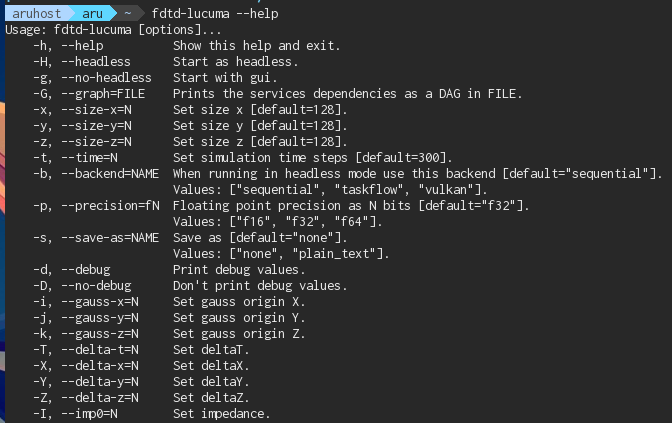
\includegraphics[width=1\textwidth]{images/cli.png}
	\caption{Fdtd Lucuma's CLI's arguments}
	\label{fig:fdtd_lucuma_cli}
\end{figure}

\subsection{CLI examples}

\inputminted[bgcolor=codeBg, tabsize=4, breaklines=true, linenos=true]{bash}{\subfix{cli-examples.sh}}

\section{GUI frontend}
An interactive interface made with Dear ImGui using it's Vulkan and SDL3 implementations.
It supports multiple independent simulations each one with it's own private EnTT registry for easier parallelism.
Plus it allows the user to add or modify the simulation's objects in real time.
While also having a heatmap visualizer for each component of the electric and magnetic fields.

\begin{figure}[H]
	\centering
	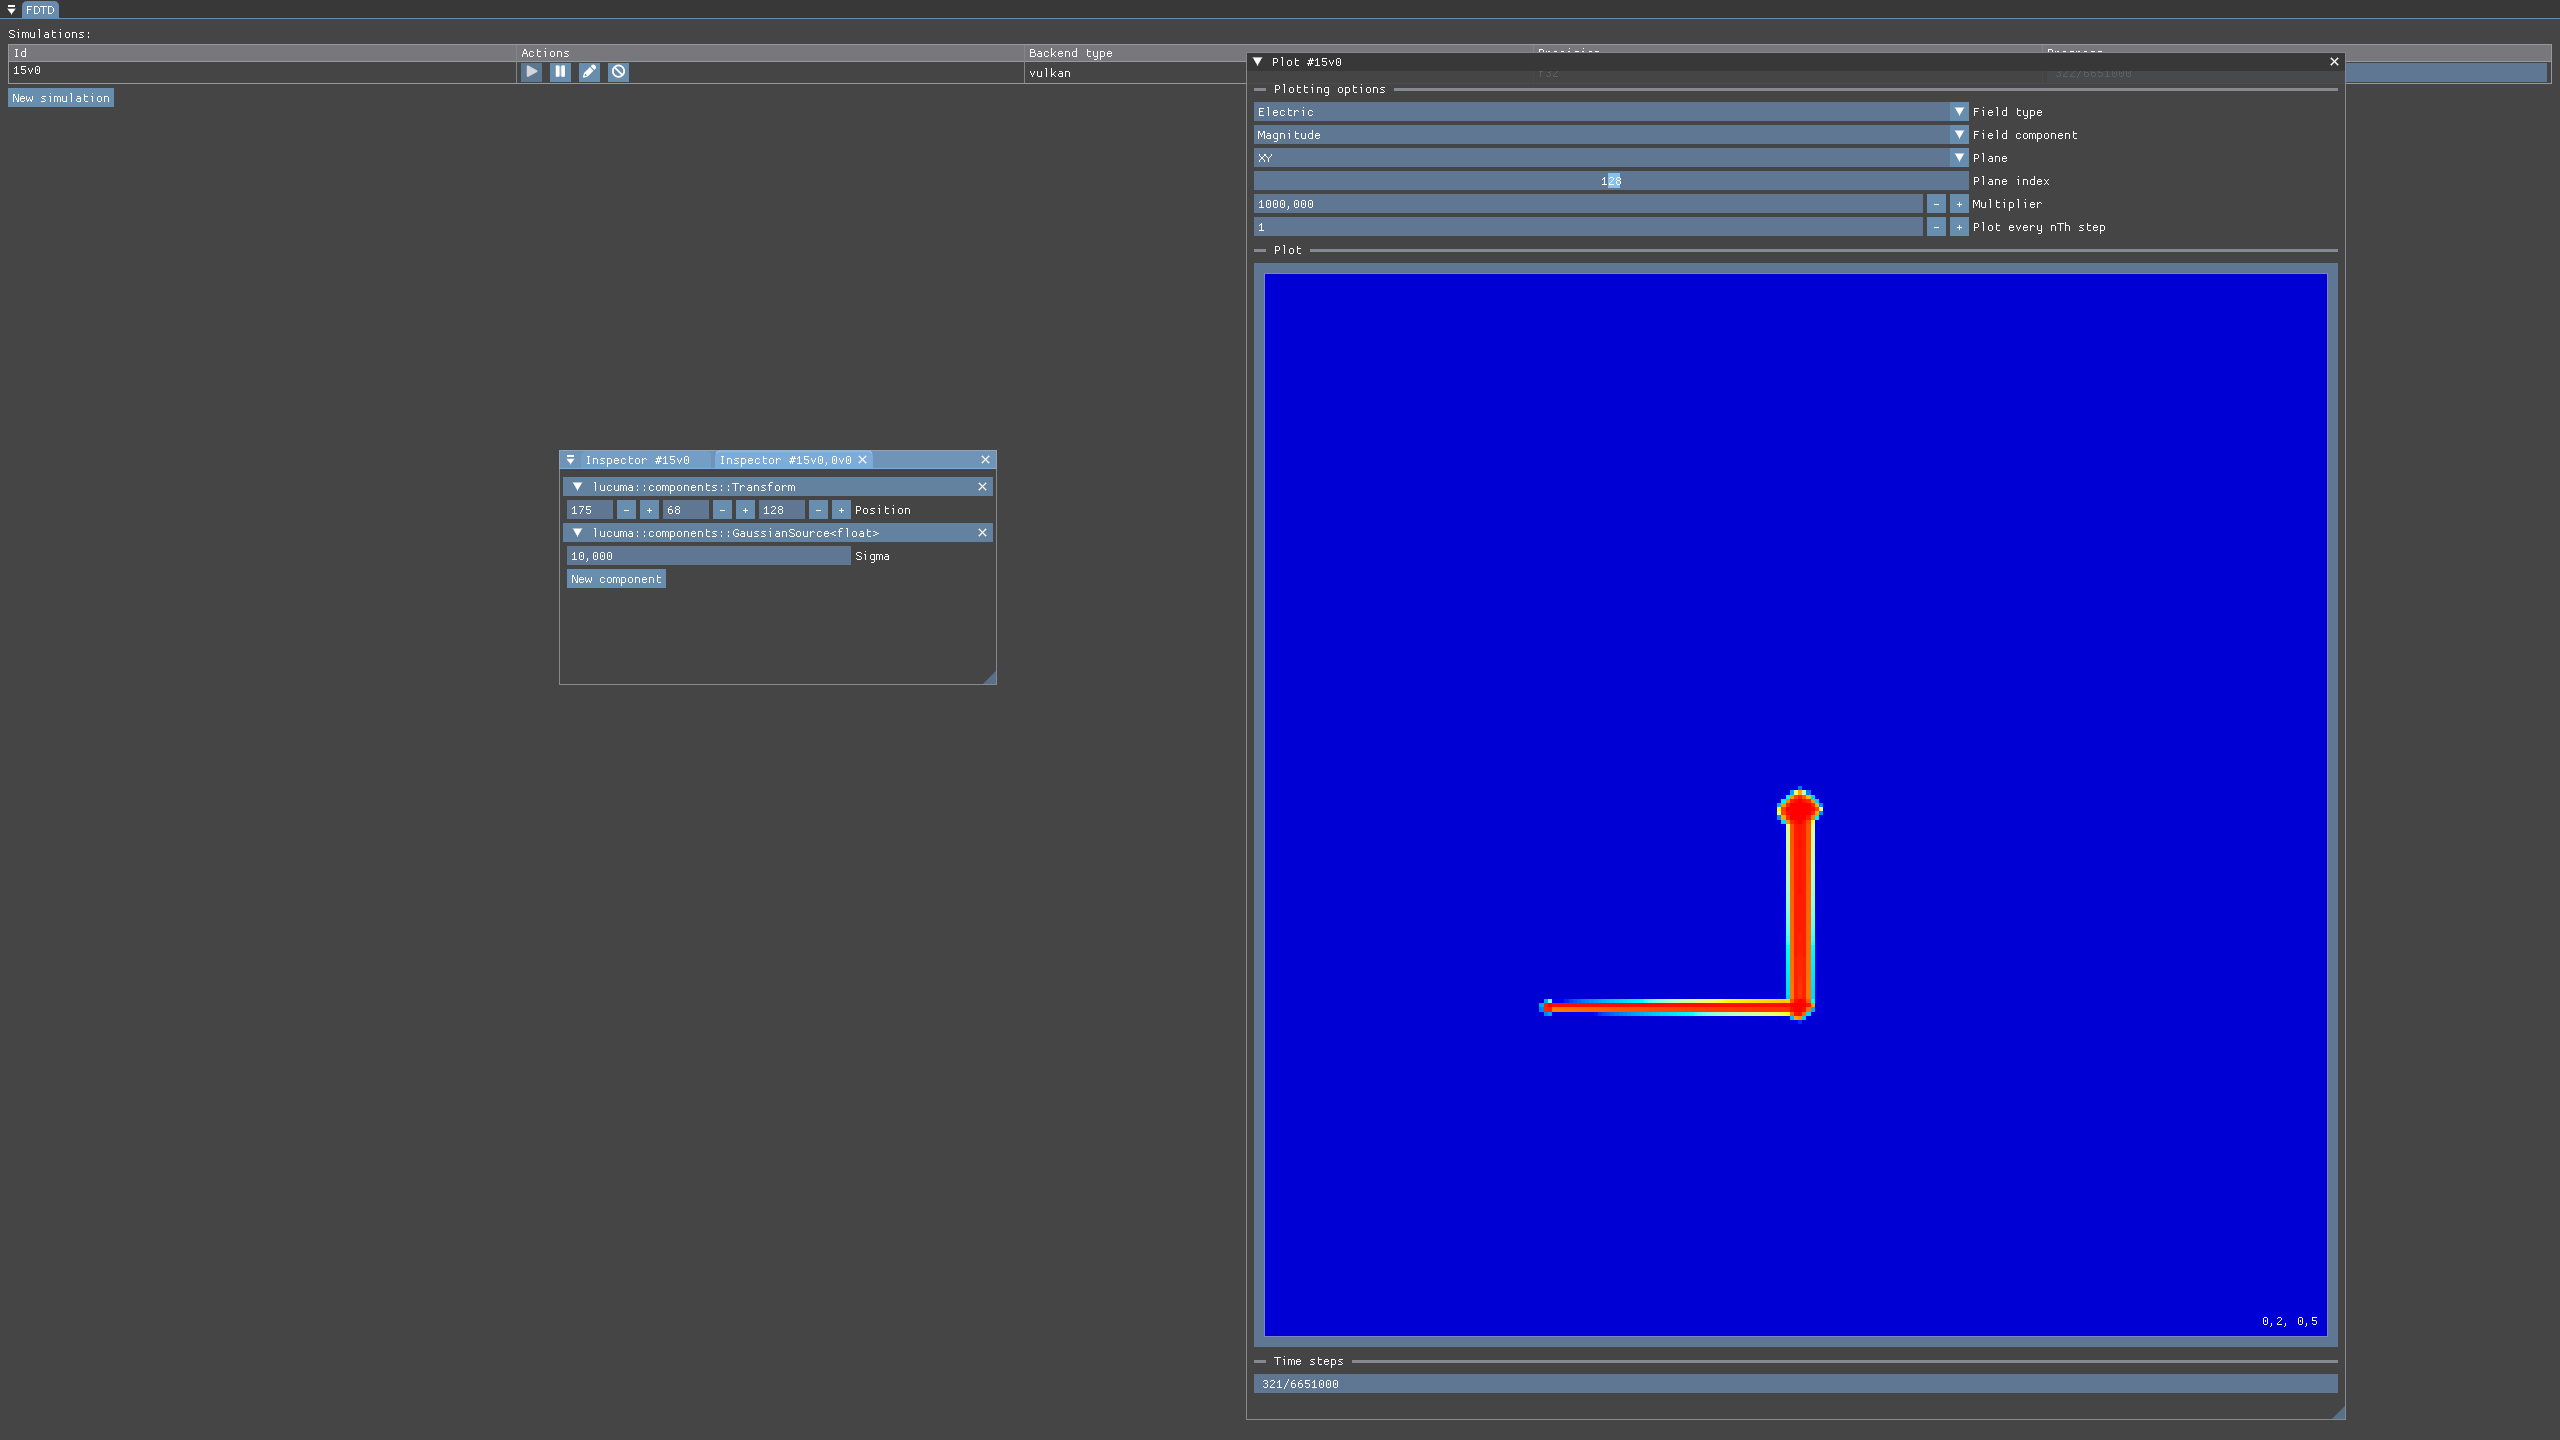
\includegraphics[width=1\textwidth]{images/moving_source.png}
	\caption{Fdtd Lucuma's GUI with a sigle gaussian source that was manually moved}
	\label{fig:fdtd_lucuma_gui}
\end{figure}


\section{CPU backends}
\subsection{Sequential}
The Sequential backend is the simplest of the three.
At each step, as shown in Figure \ref{fig:fdtd_lucuma_flow}, it updates each $\{x,y,z\}$ component of the magnetic field \blackcirclerefsection{\getrefnumber{sec:flow}:step:magnetic}, then the components of the electric field \blackcirclerefsection{\getrefnumber{sec:flow}:step:electric}, then it applies each source that exists in the EnTT registry \blackcirclerefsection{\getrefnumber{sec:flow}:step:sources} and finally the boundary conditions of each top and bottom of each component \blackcirclerefsection{\getrefnumber{sec:flow}:step:abc}.

\subsection{Parallel}
The parallel backend reuses most of the code from the sequential backend.
But it uses Taskflow to create a coarse task graph.
By wrapping each field component, source and boundary update in a task.
Then it creates a directed graph from all the tasks and their dependencies.
This allows for each component of the field updates to be parallelized as they do not have dependencies on each other.

\begin{figure}[H]
	\centering
	\begin{tikzpicture}[
			transform shape,
			node distance=2cm
		]

		\node[circle, draw] (Hx) {$H_x$};
		\node[circle, draw, below of=Hx] (Hy) {$H_y$};
		\node[circle, draw, below of=Hy] (Hz) {$H_z$};
        
		\node[circle, draw, right of=Hy] (H) {$H$};

		\node[circle, draw, right of=H] (Ey) {$E_y$};
		\node[circle, draw, above of=Ey] (Ex) {$E_x$};
		\node[circle, draw, below of=Ey] (Ez) {$E_z$};
        
		\node[circle, draw, right of=Ey] (E) {$E$};
        
		\node[circle, draw, right of=E] (Sources) {$Sources$};
		\node[circle, draw, right of=Sources] (ABC) {$ABC$};

		\draw[arrow] (Hx) -- (H);
		\draw[arrow] (Hy) -- (H);
		\draw[arrow] (Hz) -- (H);
        
		\draw[arrow] (H) -- (Ex);
		\draw[arrow] (H) -- (Ey);
		\draw[arrow] (H) -- (Ez);
        
		\draw[arrow] (Ex) -- (E);
		\draw[arrow] (Ey) -- (E);
		\draw[arrow] (Ez) -- (E);

		\draw[arrow] (E) -- (Sources);
		\draw[arrow] (Sources) -- (ABC);
        

	\end{tikzpicture}
	\caption{Tasks and dependencies of a time step}
	\label{fig:taskflow_graph}
\end{figure}


\section{Vulkan backend}
The Vulkan backend accelerates the simulation by delegating the field updates to a GPU in a vendor agnostic way.
Unlike the previous backends, to use Vulkan a lot of boilerplate is needed.
At startup time this backend instantiates an internal Vulkan Compute service, which in turn instantiates many Vulkan related services.
Which are the following listed in order of construction:
\begin{itemize}
	\item \texttt{lucuma::services::vulkan::Context}
	\item \texttt{lucuma::services::vulkan::Core}
	\item \texttt{lucuma::services::vulkan::Device}
	\item \texttt{lucuma::services::vulkan::Allocator}
	\item \texttt{lucuma::services::vulkan::ShaderLoader}
	\item \texttt{lucuma::services::vulkan::Compute}
\end{itemize}

The \texttt{Context} service holds the \texttt{vulkan::raii::Context} used to create all raii\footnote{Almost all the handles used by the services are raii. For conciseness they will be refered using their C equivalents.} Vulkan objects.
\texttt{Core} holds the \texttt{VkPhysicalDevice} and \texttt{VkInstance} and checks if the physical device is suitable by having all the required extensions and layers. \texttt{Device} uses the physical device to create and hold the \texttt{VkDevice} while also querying and selecting the best queue families for compute, graphics and presenting.
On the other hand \texttt{Allocator} is a wrapper around Vulkan Memory Allocator\citep{vma} that can be used to allocate \texttt{VkBuffer}s.
\texttt{ShaderLoader} is used to create \texttt{VkShaderModule}s from a file path. Which in turn are used to create compute or graphics \texttt{VkPipeline}s.

The \texttt{Compute} service holds the \texttt{VkQueue} and \texttt{VkCommandPool} used to send compute commands to the GPU.
When the simulation starts or when the any of it's objects change, the backend, by using \texttt{Compute}'s \texttt{createSimpleCommandBuffer()} and \texttt{createPipeline()}, creates or recreates a single \texttt{VkCommandBuffer} and multiple \texttt{VkPipeline} and \texttt{VkBuffer}s.
The backend at each simulation step resets the \texttt{VkCommandBuffer}.
Then at each substep
\blackcirclerefsection{\getrefnumber{sec:flow}:step:magnetic},
\blackcirclerefsection{\getrefnumber{sec:flow}:step:electric},
\blackcirclerefsection{\getrefnumber{sec:flow}:step:sources} and
\blackcirclerefsection{\getrefnumber{sec:flow}:step:abc}
fills it with \texttt{vkCmdBindPipelines}, \texttt{vkCmdBindDescriptorSets}, \texttt{vkCmdPushConstants} commands and
finally \texttt{vkCmdDispatch} to execute them.
To ensure proper synchronization between dispatches the backend uses \texttt{vkCmdPipelineBarrier2} between fields.
Finally the backend submits the commands, waits until the work finishes and continues with the next step.

\subsection{Dispatch example}

\inputminted[bgcolor=codeBg, tabsize=4, breaklines=true, linenos=true, escapeinside=||]{cpp}{\subfix{gauss.cpp}}


The function in line \ref{code:dispatch} fills the \texttt{VkCommandBuffer} with the commands needed to apply the gaussian sources to a component \texttt{Ec} of the electric field.
First it sets the push constants.
Then in line \ref{code:iterate} it iterates all entities that have the \texttt{Transform} and \texttt{GaussianSource} components to fill the \texttt{sourceSsbos} vector with only the needed data.
Which in turn is sent to the 

% TODO:
% - It has a lot of boilerplate.
% - Vulkan shanenigans for photonics.
% - How to use (EnTT) Entity Component System to represent a simulation and its objects
% - Vulkan Julia?

%\section{Benchmarks}

\end{document}
